\documentclass[a4paper,10pt]{bxjsarticle}
\usepackage[dvipdfmx]{graphicx}
\usepackage{url}
\usepackage{amsmath}
\usepackage{amssymb}
\usepackage{amsfonts}
% \usepackage{here}

\title{プログラム演習 課題3}
\date{ }

\begin{document}

\maketitle

% \section*{section}

比誘電率$\epsilon_r$、厚さ$a$の誘電体スラブに沿ってz方向伝搬するTMモードの分散関係式を求める。

\begin{figure}[h]
    \centering
    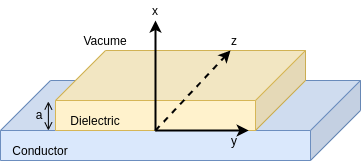
\includegraphics[width=0.7\textwidth]{fig.png}
    \caption{}
    \label{fig:1}
\end{figure}

$\rho = 0$とすると、Maxwell方程式は
\begin{eqnarray}
    \nabla \times \mathbb{E} &=& - \frac{\partial}{\partial t} \mathbb{B} \\
    \nabla \times \mathbb{B} &=&  \frac{\partial}{\partial t} \mu \epsilon \mathbb{E} \\
    \nabla \cdot \mathbb{E} &=& \frac{\rho}{\epsilon} = 0
\end{eqnarray}
となる。

(1)の両辺の回転をとる
\begin{align*}
    \nabla \times \left(\nabla \times \mathbb{E}\right)
        &= - \frac{\partial}{\partial t} \nabla \times \mathbb{B} \\
    \nabla \left(\nabla \cdot \mathbb{E}\right) - \nabla^2 \mathbb{E}
        &= - \frac{\partial}{\partial t} \frac{\partial}{\partial t} \mu \epsilon \mathbb{E} \\
    - \nabla^2 \mathbb{E}
        &= - \mu \epsilon \frac{\partial^2}{\partial t^2} \mathbb{E} \\
    \nabla^2 \mathbb{E} - \mu \epsilon \frac{\partial^2}{\partial t^2} \mathbb{E}
        &= 0 \qquad \cdots Holmheltz \ eq \\
\end{align*}

$\mathbb{E} \propto e^{j\omega t}$より、$\frac{\partial}{\partial t} = j\omega$とおくと
Holmheltz方程式は
$$
\nabla^2 \mathbb{E} + \omega^2 \mu \epsilon \mathbb{E} = 0
$$

$\mathbb{E}$のz成分について
$$
\left( 
    \frac{\partial^2}{\partial x^2} 
    + \frac{\partial^2}{\partial y^2} 
    + \frac{\partial^2}{\partial z^2} 
\right) E_z
+ \omega^2 \mu \epsilon E_z
= 0
$$

z方向伝搬より $$E_z \propto e^{-\gamma z} = e^{-(\alpha + j \beta)z}$$ \\
無損失を仮定すると $\alpha = 0$なので $$E_z \propto e^{ -j \beta z}$$ \\
したがって、$ \frac{\partial}{\partial z} = -j \beta $ とすると、
Holmheltz方程式は
\begin{align*} 
\left( 
    \frac{\partial^2}{\partial x^2} 
    + \frac{\partial^2}{\partial y^2} 
    - \beta^2 
    + \omega^2 \mu \epsilon
\right) E_z
&= 0 \\
\left( 
    \frac{\partial^2}{\partial x^2} 
    + \frac{\partial^2}{\partial y^2} 
    + k_c^2
\right) E_z
&= 0 \qquad
\because \ k_c^2 = \omega^2 \mu \epsilon - \beta^2 \\
\end{align*}

また、y方向に無限なスラブと仮定すると$\frac{\partial}{\partial y} = 0$となる。
\begin{align*} 
    \left( 
        \frac{\partial^2}{\partial x^2} + k_c^2
    \right) E_z
    &= 0 \\
\end{align*}

したがって、
$$ E_z = A \sin k_c x + B \cos k_c x \qquad (A,B : const) $$

境界条件 $x = 0$で$E_z = 0$ より
\begin{align*}
    E_z|_{x=0} &= A \sin k_c 0 + B \cos k_c 0 \\
             &= B \\ 
             &= 0 \\
    E_z &= A \sin k_c x
\end{align*}

また真空中の場合、
電場のz成分についてのHolmheltz方程式は以下のようになる。
\begin{align*}
    \left( 
        \frac{\partial^2}{\partial x^2} 
        + \frac{\partial^2}{\partial y^2} 
        - \beta^2
    \right) E_z
    + \omega^2 \mu_0 \epsilon_0 E_z
    & = 0
\end{align*}

誘電体スラブ中と同様に$\frac{\partial}{\partial y} = 0$とすると
\begin{align*}
    \left( 
        \frac{\partial^2}{\partial x^2} 
        + \omega^2 \mu_0 \epsilon_0 - \beta^2 
    \right) E_z
    & = 0 \\
    \left( 
        \frac{\partial^2}{\partial x^2} 
        + k_0^2
    \right) E_z
    & = 0 \qquad
    \because \ k_0^2 = \omega^2 \mu_0 \epsilon_0 - \beta^2 \\
\end{align*}

$k_0^2 > 0$の場合、
\begin{align*}
    E_z &= C e^{j k_0 x} \\
        &= C \cos k_0 x + j C \sin k_0 x
\end{align*}

$k_0^2 < 0$の場合、
$k_0^2 = - k_0^{\prime 2} = - \omega^2 \mu_0 \epsilon_0 + \beta^2$ とすると
\begin{align*}
    \left( 
        \frac{\partial^2}{\partial x^2} 
        + k_0^2
    \right) E_z
    & =
    \left( 
        \frac{\partial^2}{\partial x^2} 
        - k_0^{\prime 2}
    \right) E_z
    = 0 \\
    E_z &= C^\prime e^{- k_0^\prime x}
\end{align*}

$x=a$での境界条件より、真空中の電場と誘電体中の電場は連続なので、

$k_0^2 < 0$のとき
\begin{align*}
    A \sin k_c a & = C^\prime e^{- k_0 a} \\
    \sin k_c a & = \frac{C^\prime}{A} e^{- k_0 a} \\
    k_c a & = \sin^{-1} \left( \frac{C^\prime}{A} e^{- k_0 a} \right) \\
    k_c & = \frac{1}{a} \sin^{-1} \left( \frac{C^\prime}{A} e^{- k_0 a} \right) \\
    \omega^2 \mu \epsilon - \beta^2 &= 
        \left[ 
            \frac{1}{a} \sin^{-1} \left( C_0 e^{- k_0 a} \right)
        \right]^2 \qquad
    \because \ C_0 = \frac{C^\prime}{A}
\end{align*}

$k_0^2 > 0$のとき
\begin{align*}
    E_z &= C e^{j k_0 x} \\
        &= C \cos k_0 x + j C \sin k_0 x
\end{align*}

\begin{align*}
    A \sin k_c a &= C \cos k_0 a + j C \sin k_0 a \\
    \\
    A \sin k_c a &= C \cos k_0 a \\
    C \sin k_0 a &= 0 \\
    \\
    A \sin (\omega^2 \mu \epsilon a - \beta^2a)
        &= C \cos (\omega^2 \mu_0 \epsilon_0 a - \beta^2a) \\
    A \sin (\omega^2 \mu \epsilon a) \cos (\beta^2a)
        - A \sin (\beta^2a) \cos (\omega^2 \mu \epsilon a)
    &= C \cos (\omega^2 \mu_0 \epsilon_0 a) \cos (\beta^2a) 
        + C \sin (\omega^2 \mu_0 \epsilon_0 a) \sin (\beta^2a) \\
    \cos (\beta^2a) \left[
        A \sin (\omega^2 \mu \epsilon a) - C \cos(\omega^2 \mu_0 \epsilon_0 a)
    \right]
    &= \sin (\beta^2a) \left[
        A \cos (\omega^2 \mu \epsilon a) + C \sin (\omega^2 \mu_0 \epsilon_0 a)
    \right] \\
    \frac{\sin (\beta^2a)}{\cos (\beta^2a)}
    &= \frac{A \sin (\omega^2 \mu \epsilon a) - C \cos(\omega^2 \mu_0 \epsilon_0 a)}{A \cos (\omega^2 \mu \epsilon a) + C \sin (\omega^2 \mu_0 \epsilon_0 a)} \\
    \tan \beta^2a
    &= \frac{A \sin (\omega^2 \mu \epsilon a) - C \cos(\omega^2 \mu_0 \epsilon_0 a)}{A \cos (\omega^2 \mu \epsilon a) + C \sin (\omega^2 \mu_0 \epsilon_0 a)} \\
    \beta^2a
    &= \tan^{-1} \left[
        \frac{A \sin (\omega^2 \mu \epsilon a) - C \cos(\omega^2 \mu_0 \epsilon_0 a)}{A \cos (\omega^2 \mu \epsilon a) + C \sin (\omega^2 \mu_0 \epsilon_0 a)}
    \right] \\
\end{align*}

%===========================================================================
% \cite{aaa}
% \begin{thebibliography}
%     \bibitem{aaa} aaa \url{url}
% \end{thebibliography}

% \begin{table}[htb]  
%     \centering
%     \caption{table}
%     \begin{tabular}{|c|c|c|} \hline
%         a & b & c \\\hline
%         1 & 2 & 3 \\\hline
%     \end{tabular}
% \end{table}

%   \begin{figure}[h]
%       \centering
%       \includegraphics[width=0.7\textwidth]{  }
%       \caption{}
%       \label{fig:}
%   \end{figure}
  
\end{document}